%
%   Prof. Dr. Julian Reichwald
%   auf Basis einer Vorlage von Prof. Dr. Jörg Baumgart
%   DHBW Mannheim
%
%	ACHTUNG: Für das Erstellen des Literaturverzeichnisses wird das modernere Paket biblatex
%			 in Kombination mit biber verwendet -- nicht mehr das ältere BibTex!
% 			 Bitte stellen Sie ggf. Ihre TeX-Umgebung
% 			 entsprechend ein (z.B. TeXStudio: Einstellungen --> Erzeugen --> Standard Bibliographieprogramm: biber)
%

\documentclass[
	12pt, % defaut=12
	BCOR=5mm,
	DIV=12, % ca 3.5cm margins % default=12
	headinclude=on,
	footinclude=off,
	parskip=half,
	bibliography=totoc,
	listof=entryprefix,
	toc=listof,
	number=noenddot,
	plainfootsepline]{scrreprt}

%	Konfigurationsdatei einbinden
% !TEX root = ../master.tex

%-------------------
% 		HYPERREF
%-------------------

\usepackage[hidelinks=true]{hyperref}
 % hidelinks=true verhindert rote Ränder bei Links im Dokument.

% URLs im Fließtext
\newcommand{\urlinline}[1]{\textsf{\footnotesize{\url{{#1}}}}}

% Zwei eigene Befehle zum Setzen von Autor und Titel. Ausserdem werden die PDF-Informationen richtig gesetzt.
\newcommand{\titel}[1]{\def\dertitel{#1}\hypersetup{pdftitle={#1}}}
\newcommand{\autor}[1]{\def\derautor{#1}\hypersetup{pdfauthor={#1}}}
\newcommand{\ort}[1]{\def\derort{#1}}

%-----------------------------------
%		SCHRIFT UND ENCODING
%-----------------------------------
\usepackage[T1]{fontenc}
\usepackage[utf8]{inputenc}

\usepackage{setspace}
%\onehalfspacing
%TODO use this spacing

%---------------------------
%		BERECHNUNGEN
%---------------------------
\usepackage{calc} % Used for extra space below footsepline

%---------------------------------
%		SPRACHEINSTELLUNGEN
%---------------------------------
% Voreinstellungen für Deutsch und Englisch. Die nicht verwendete Sprache ist auszukommentieren.
% DEUTSCH
%\usepackage[ngerman]{babel}
%\usepackage[german=quotes]{csquotes}

%ENGLISCH
\usepackage[english, ngerman]{babel}
\usepackage{csquotes} % Richtiges Setzen der Anführungszeichen mit \enquote{}

%----------------------------
%		BIBLIOGRAFIE
%----------------------------
% Voreinstellungen für Fußnotenzitate (Autor-Jahr), IEEE-Standard, Alphabetic-Stil und Havard-Stil. Die nicht verwendeten Stile müssen auskommentiert werden

%\usepackage[backend=biber, autocite=footnote, style=authoryear, dashed=false]{biblatex}		% Fußnotenzitate
\usepackage[backend=biber, autocite=inline, style=ieee]{biblatex}							% IEEE-Stil
%\usepackage[backend=biber, autocite=inline, style=alphabetic]{biblatex}					% Alphabetic-Stil
%\usepackage[backend=biber, autocite=inline, style=authoryear, dashed=false]{biblatex}		% Harvard-Stil
%\usepackage[backend=biber, autocite=inline, style=apa]{biblatex}							% APA-Stil

% Fußnotenzitate mit YYYY-MM-DD in Bibliographie
% \usepackage[backend=biber, autocite=footnote, style=authoryear, dashed=false, urldate=edtf, date=edtf, seconds=true]{biblatex}

% Zum Zählen der Fußnoten über Kapitel hinaus
\usepackage{chngcntr}
\counterwithout{footnote}{chapter}

\DefineBibliographyStrings{ngerman}{  %Change u.a. to et al. (german only!)
	andothers = {{et\,al\adddot}},
}

\setlength{\bibparsep}{\parskip}		%add some space between biblatex entries in the bibliography
\addbibresource{adds/bibliography.bib}	%Add file bibliography.bib as biblatex resource

%----------------------
%		ACRONYME
%----------------------
%%%
%%% WICHTIG: Installieren Sie das neueste Acronyms-Paket!!!
%%%
\makeatletter
\usepackage[printonlyused]{acronym}
\@ifpackagelater{acronym}{2015/03/20}
  {%
    \renewcommand*{\aclabelfont}[1]{\textbf{\textsf{\acsfont{#1}}}}
  }%
  {%
  }%
\makeatother

%--------------------
%		GLOSSAR
%--------------------
%\usepackage[toc]{glossaries}					% für Seitenreferenzen im Glossar
\usepackage[toc, nonumberlist]{glossaries}		% ohne Seitenreferenzen im Glossar

%---------------------
%		LISTINGS
%---------------------
\usepackage{listings}
% Listings formatieren
\renewcommand{\lstlistlistingname}{List of Listings}
\lstset{numbers=left,
	numberstyle=\tiny,
	captionpos=b,
	breaklines=true,
	basicstyle=\linespread{0.8}\ttfamily\small}

%-------------------------------
%		ZUSÄTZLICHE PAKETE
%-------------------------------
\usepackage{lipsum}				% Blindtext
\setlipsumdefault{1-4}
\usepackage[pdftex]{graphicx} 			% verschiene Bildformate einbinden
\usepackage{pdfpages}		% PDF einbinden
\usepackage{varioref} 	% schönere Referenzen über \vref{}
\usepackage{caption}			% schönere Überschriften
\usepackage{booktabs}			% bessere Tabs
\usepackage{array}
\newcolumntype{P}[1]{>{\raggedright\arraybackslash}p{#1}}

% bessere Tabellen
\setlength{\tabcolsep}{10pt}
\renewcommand{\arraystretch}{1.5}

% resource folder einbinden
\graphicspath{ {resources/} }

%--------------------------
%		Tikz diagram library
%--------------------------
\usepackage{tikz}
\usetikzlibrary{arrows,decorations.pathmorphing,backgrounds,fit,positioning,shapes.symbols,chains}

%--------------------------
%		TpX used packages
%--------------------------
\usepackage{color}
\DeclareGraphicsExtensions{.pdf,.png,.jpg,.jpeg,.mps}
\usepackage{pgf}
\usepackage{epic,bez123}
\usepackage{floatflt}% package for floatingfigure environment
\usepackage{wrapfig}% package for wrapfigure environment

%-------------------------
%		ALGORITHMEN
%-------------------------
\usepackage{algorithm}
\usepackage{algpseudocode}
\renewcommand{\listalgorithmname}{List of Algorithms}
\floatname{algorithm}{algorithm}

%-------------------------
%		SCHRIFTART
%-------------------------
% Entweder Latin Modern oder Times / Helvetica
\usepackage{lmodern} %Latin modern font
%\usepackage{mathptmx}  %Helvetica / Times New Roman fonts (2 lines)
%\usepackage[scaled=.92]{helvet} %Helvetica / Times New Roman fonts (2 lines)

%------------------------------------
%		KOPFZEILE / FUßZEILE
%------------------------------------
%	   ACHTUNG! Einige einstellungen werden in master.tex erneut verändert
\RequirePackage[automark,headsepline,footsepline]{scrpage2}
\pagestyle{scrheadings}
\renewcommand*{\pnumfont}{\upshape\sffamily}
\renewcommand*{\headfont}{\upshape\sffamily}
\renewcommand*{\footfont}{\upshape\sffamily}
\renewcommand{\chaptermarkformat}{}

\clearscrheadfoot

% using cfoot centers the header
% use ofoot for outer side, especially with documentclass[twoside]
\cfoot[\rule{0pt}{\ht\strutbox+\dp\strutbox}\pagemark]{\rule{0pt}{\ht\strutbox+\dp\strutbox}\pagemark}

\ohead{\headmark}

%TODO: fix footer

%-----------------------------------
%		Fix Headheight
%-----------------------------------
\setlength{\headheight}{1.1\baselineskip}

%\input{adds/glossary}

%\makeglossaries

\begin{document}

%----------------------------------------
% Titel und Autor der Arbeit hier angeben
%----------------------------------------
\titel{Volume Recognition in Video Images for Movement Optimization of Passenger Elevators}
\autor{Felix Stegmaier}
\ort{Stuttgart}

\singlespacing

% !TEX root = ../master.tex
\begin{titlepage}

\begin{minipage}{\textwidth}
		\vspace{-2cm}
		\noindent
		\raisebox{-0.5\height}{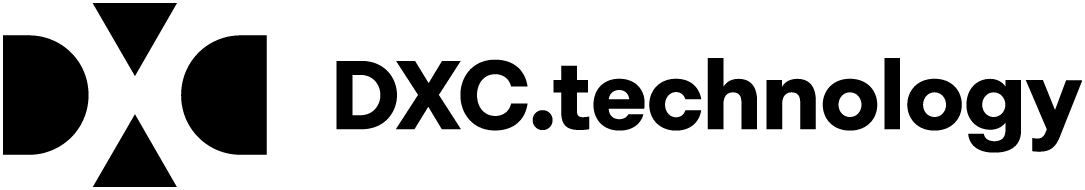
\includegraphics[width=7cm, keepaspectratio]{dxc_logo}}
		\hfill
		\raisebox{-0.5\height}{
\includegraphics[width=5cm, keepaspectratio]{dhbw_logo}}
\end{minipage}

\enlargethispage{20mm}

\sffamily
\begin{center}
    \vspace*{24mm}  {\large\textbf{\dertitel}}       \\
    \vspace*{12mm}  {\large\textbf{Bachelor Thesis}}        \\
    \vspace*{24mm}   for the course of study         \\
    \vspace*{3mm}   {\large\textbf{Computer Science}} \\
    \vspace*{3mm}   at the                         \\
    \vspace*{3mm}   {\large\textbf{Baden-Wuerttemberg Cooperative State University Stuttgart}}  \\
    \vspace*{12mm}  by                              \\
    \vspace*{3mm}   {\large\textbf{\derautor}}      \\
    \vspace*{12mm}  03 September 2018 \\

\vfill

\begin{minipage}{\textwidth}

\begin{tabbing}
	Scientific Supervisor: \hspace{1.85cm} \= \kill
	Project Period: \` 12 Weeks \\[1.5mm]
	Student ID, Course: \` 6079153, TINF15A\\[1.5mm]
	Company: \` DXC Technology, Böblingen\\[1.5mm]
	Supervisor: \` Julia Baumhauer, Executive Master of Arts\\[1.5mm]
	Scientific Supervisor: \` Prof. Dr. Bernd Schwinn \\[1.5mm]

\end{tabbing}
\end{minipage}

\end{center}

\end{titlepage}


\pagenumbering{Roman} % Römische Seitennummerierung
\normalfont

%----------------------------------------
% Verzeichnisse - nicht benötige Verzeichnisse bitte auskommentieren / löschen.
%----------------------------------------

\onehalfspacing
\pagestyle{scrheadings}
%   Sperrvermerk
%% !TEX root = ../master.tex
\chapter*{Confidentiality Notice}
\thispagestyle{scrheadings}
This work as a whole or in part may
not be disclosed to persons outside of the exam and evaluation process,
provided that no other approval is given by the training institution or the author.
\cleardoublepage


\onehalfspacing
\pagestyle{scrheadings}
% Ehrenwörtliche Erklärung
% !TEX root = ../master.tex
\clearpage

\selectlanguage{ngerman}

\chapter*{Erklärung}
\thispagestyle{scrheadings}
Ich versichere hiermit, dass ich meine Bachelorarbeit mit dem Thema \textit{\dertitel} selbstständig verfasst und keine anderen als die angegebenen Quellen und Hilfsmittel
benutzt habe.
Ich versichere zudem, dass die eingereichte elektronische Fassung mit der gedruckten Fassung
übereinstimmt.

\vspace{3cm}
\derort, \today
\vspace{3em}

\rule{6cm}{0.4pt}\\
\derautor

\clearpage

\selectlanguage{english}

\chapter*{Declaration of Authorship}
\thispagestyle{scrheadings}

% Wird die folgende Zeile auskommentiert, erscheint die ehrenwörtliche
% Erklärung im Inhaltsverzeichnis.

% \addcontentsline{toc}{chapter}{Ehrenwörtliche Erklärung}

I hereby declare:

\begin{itemize}
	\item that this paper with the title \textit{\dertitel} is my own work and
	\item that I have not used any other sources or assistance than declared here.
	\item that I have not submitted the paper as a whole or in part for an degree at any university
		or institution before.
	\item that I have not published this paper before.
	\item Furthermore I confirm, that the presented electronical version of this paper
		is identical to the printed version.
\end{itemize}
I am aware, that an incorrect declaration will be followed by legal measures.

\vspace{3cm}
\derort, \today
\vspace{3em}

\rule{6cm}{0.4pt}\\
\derautor



\singlespacing
\pagestyle{scrheadings}
%	Kurzfassung
% !TEX root = ../master.tex

\selectlanguage{ngerman}

\chapter*{Abstract}

\begingroup
  \begin{table}[h!]
    \setlength\tabcolsep{0pt}
    \begin{tabular}{p{3.5cm}p{10.0cm}}
      Titel & \dertitel \\
      Autor: & \derautor \\
    \end{tabular}
  \end{table}
\endgroup

Fahrstühle bewegen Menschen -- jeden Tag.
Die Fahrwege einer modernen Personenfahrstuhlanlage hängen ab von den Personen, die in jeder Etage auf ihre Beförderung zu unterschiedlichen Zielen warten sowie den Personen im Aufzug, die bereits auf dem Weg zu einer Zieletage sind. Aktuelle Systeme versuchen durch Angabe des Ziels beim Rufen des Aufzuges die Wege der Kabine für eine gleichverteilte und im Mittel schnelle Beförderung zu planen und Wartezeiten zu verringern sowie die Auslastung der Anlage zu optimieren.

In dieser Arbeit werden Möglichkeiten ergründet, diesen Prozess durch die Verwendung von Kamerasystemen in den Kabinen und vor den Einlässen zu unterstützen, indem durch Personen- und Objekterkennung die Anzahl der Passagiere und Wartenden sowie deren Platzbedarf und der Freiraum in der Kabine analysiert wird. 
Der Fokus liegt dabei auf der Analyse der benötigten und freie Volumina.
Dies umfasst eine Implementierung eines entsprechenden Bilderkennungssystems und eine modellhafte Darlegung eines Fahrstuhlsystems, das dieses verwendet.

Das entwickelte Bilderkennungssystem verwendet mehrere Kameras 
und nutzt die Hintergrundsubtraktionstechnik um die Position von Personen und Objekten in der Kabine zu erfassen.
Ein shilhouettenbasierter Volumenschnitt wird durchgeführt um das eingenommene Volumen der Anwesenden zu erkennen.
Die so gewonnenen Daten können in einem angepassten Steuerungsalgorithmus für Aufzugsysteme genutzt werden, 
der großen Objekten in der Kabine Vorrang gewärt, um diese schneller zuzustellen.
Da diese Objekte die Kabine für andere Fahrgäste blockieren,
kann dies die Anzahl der beförderten Objekte erhöhen, 
was mit einer durchgeführten Simulation untermauert wird.
Eine solche Modifikation der Kotrollalgorithmus kann für Umfelder sinnvoll sein, in denen Passagiere und Objekte um Beförderung im Aufzug konkurrieren. 

\selectlanguage{english}

\chapter*{Abstract}

\begingroup
  \begin{table}[h!]
    \setlength\tabcolsep{0pt}
    \begin{tabular}{p{3.5cm}p{10.0cm}}
      Title & \dertitel \\
      Author: & \derautor \\
    \end{tabular}
  \end{table}
\endgroup

\hspace{2cm}

Elevators move people -- every day.
The movement of a modern passenger elevator system depends on the persons on
each floor waiting to be transported to different destinations as well as the
passengers inside the elevator already on the way to their terminal location.
Recent systems try to optimize the movement of the elevator by utilizing
destination dispatch controls on each floor in such a way that travel
waiting times for passengers are minimized and the utilization of the elevator
is maximized.

This paper explores possibilities to support this process by the usage of
camera systems within the cabin and in front of the entrances which analyze
the amount and spatial needs of people waiting for the elevator as well as
currently occupying it.
The system employs techniques from the object and person recognition
from the field of computer vision.
The focus of the automated analysis is the spatial volume needed to
transport the passengers.
The work done for this paper includes an implementation of an appropriate
image recognition system and an exemplary outline of an elevator system
that uses such a system.

The developed visual recognition system uses a multi-view camera set-up with the techniques of background subtraction to register the positions of passengers and objects in the elevator cabin.
The technique of silhouette-based volume intersection is used to detect the volume that these entities take up.
The data gathered by this system can be used for an elevator scheduling algorithm which gives priority to the delivery of large objects in the cabin, which blocks the space for other passengers.
A conducted simulation yields that this approach can improve the 
amount of delivered objects, which can be beneficial in an environment where passengers and cargo objects need to be moved likewise. 



\onehalfspacing
\pagestyle{scrheadings}
% Vorangehende Notitzen
% !TEX root = ../master.tex
\clearpage
\chapter*{Preliminary Notes}
\label{chap:prenotes}
\thispagestyle{scrheadings}

\paragraph{Gender Neutrality}
This paper is written in gender neutral language.
Any person is addressed using the singular \emph{they}.
For example, instead of
``The user changes \emph{his} account settings.''
this paper writes
``The user changes \emph{their} account settings.''


\paragraph{Trademarks}
Designations from third-party vendors are used in this paper.
These designations may be trademarks or registered trademarks.
Wherever the author is aware of such trademark,
the designation will be written with an initial capital letter.

\paragraph{Formatting}
TODO which formatting are used to highlight what
\emph{Italic text}
\textbf{Bold text}
\texttt{Monospace text}
\textit{S} Symbols in Formulars


\singlespacing

%	Inhaltsverzeichnis
\begingroup
%\renewcommand*{\chapterpagestyle}{empty}
%\pagestyle{empty}
\renewcommand*{\chapterpagestyle}{scrheadings}
\pagestyle{scrheadings}
%\setcounter{tocdepth}{2} % TODO adapt if toc too long
\tableofcontents
\clearpage
\endgroup

\pagestyle{scrheadings}
\setcounter{tocdepth}{2}
%	Abbildungsverzeichnis
\listoffigures
%	Tabellenverzeichnis
\listoftables
%	Listingsverzeichnis
\lstlistoflistings
% 	Algorithmenverzeichnis
\listofalgorithms

% 	Abkürzungsverzeichnis (siehe Datei acronyms.tex!)
% !TEX root = ../master.tex
\clearpage
\chapter*{List of Acronyms}
\addcontentsline{toc}{chapter}{List of Acronyms}

%Verwendung:
%		\ac{Abk.}   --> fügt die Abkürzung ein, beim ersten Aufruf wird zusätzlich automatisch die ausgeschriebene Version davor eingefügt bzw. in einer Fußnote (hierfür muss in header.tex \usepackage[printonlyused,footnote]{acronym} stehen) dargestellt
%		\acs{Abk.}   -->  fügt die Abkürzung ein
%		\acf{Abk.}   --> fügt die Abkürzung UND die Erklärung ein
%		\acl{Abk.}   --> fügt nur die Erklärung ein
%		\acp{Abk.}  --> gibt Plural aus (angefügtes 's'); das zusätzliche 'p' funktioniert auch bei obigen Befehlen
%	siehe auch: http://golatex.de/wiki/%5Cacronym

\begin{acronym}
	\acro{API}{application programming interface}
	\acro{CPU}{central processing unit}
	\acro{CV}{Computer Vision}
	\acro{DHBW}{Baden-Wuerttemberg Cooperative State University}
	\acro{IP}{Internet Protocol}
	\acro{IT}{Information Technology}
	\acro{RAM}{Random Access Memory}
\end{acronym}


% !TEX root = ../master.tex
\clearpage
\chapter*{List of Symbols}
\addcontentsline{toc}{chapter}{List of Symbols}


\begin{tabular}{lll}
    Symbol & Unit & Description\\
    \hline
    $h$     & $cm$      & Height\\
    $h_px$  & $px$      & 
    $w$     & $cm$      & Width\\
    $d$     & $cm$      & Diameter\\
    $A$     & $cm^2$    & Area\\
    $A_px$   & $px^2$    & Pixel Area\\
    $V$     & $cm^3$    & Volume
\end{tabular}


% TODO remove this
% % !TeX root = ../master.tex
\chapter*{Commented Bibliography}

\newcommand{\parstartcite}[1]{\textbf{\citeauthor{#1}} \textsf{\citetitle{#1}} \newline}

\parstartcite{beyeler2017opencvml} is a an advanced, hands on book.
OpenCV machine learning connects the fundamental theoretical principles
behind machine learning to their practical applications in a way that focuses
on asking and answering the right questions.
This book walks you through the key elements of OpenCV
and its powerful machine learning classes,
while demonstrating how to get to grips with a range of models.
This book targets Python programmers who are already familiar with OpenCV;
this book will give you the tools and understanding required to build your
own machine learning systems, tailored to practical real-world tasks

\parstartcite{crawford2017opencvpythonvideo} is a video course for OpenCV beginners.
OpenCV is an open-source toolkit for advanced computer vision.
It is one of the most popular tools for facial recognition,
used in a wide variety of security, marketing, and photography applications,
and it powers a lot of cutting-edge tech, including augmented reality
and robotics. This course offers Python developers a detailed introduction to
OpenCV 3, starting with installing and configuring your Mac, Windows,
or Linux development environment along with Python 3.
Learn about the data and image types unique to OpenCV, and find out how to
manipulate pixels and images. Instructor Patrick W. Crawford also shows how
to read video streams as inputs, and create custom real-time video interfaces.
Then comes the real power of OpenCV: object, facial, and feature detection.
Learn how to leverage the image-processing power of OpenCV using methods like
template matching and machine learning data to identify and recognize features.

\parstartcite{rusu2011pointcloud}

\parstartcite{levine1989microwave}

\parstartcite{wang2017apple}

\parstartcite{hildebrand1997thickness}

\parstartcite{vogiatzis2010stereo}

\parstartcite{taj2010detection}

\parstartcite{hartley2004multiview}

\parstartcite{bostondiditeam2017mv3d}

\parstartcite{chen2017mv3d}

\parstartcite{saxena2007reconstruction}

\parstartcite{ge2010crowd}

\parstartcite{bayoa2009foreground}

\parstartcite{mordvintsev2013background}

\parstartcite{opencv2018histogram}

\parstartcite{reddy2013foreground}

\parstartcite{zhang2017imageprocessing}

\parstartcite{grady2017graph}

\parstartcite{inoli2014imageprocessing}

\parstartcite{sun2010groupelevator}

\parstartcite{beers2015arrivals}

\parstartcite{kwon2014sensor}


%----------------------------------------
% Start des Textteils der Arbeit
%----------------------------------------
\clearpage
\ihead{\chaptername~\thechapter} % Neue Header-Definition
\pagenumbering{arabic}  % Arabische Seitenzahlen

\onehalfspacing
\pagestyle{scrheadings}

%Einzelne Kapitel können hier eingefügt werden.
%Es ist vorgesehen alle Kapitel als eigene Dateien
% !TEX root = ../master.tex
\chapter{Introduction}
\label{chap:intro}

\section{Computer Vision and Elevators}

%\begin{figure}
%\begin{equation}
%f(x)=x^2
%\label{eqn:e2}
%\end{equation}
%\caption{Quadratic Function}
%\end{figure}

\lipsum[1-10]

TODO
- general intro to why camera vision is gaining importance in public places 
- and why elevator movement is an topic of economic interest.


\section{Context}

- andere paper referenzieren
- DXC Startup autobahn 
- startup abgesprungen

TODO

\section{Motivation}

TODO

where does the problem come from?
why is this work relevant?

\section{Goals and Boundaries}

TODO Problem Statement (maybe own section)

TODO scope and non-scope

\section{Structure of this Document}

TODO

\begin{itemize}
    \item Chapter \ref{chap:sota}
    \item Chapter \ref{chap:design}
    \item Chapter \ref{chap:impl}
    \item Chapter \ref{chap:concl}
\end{itemize}
% !TEX root = ../master.tex
\chapter{Fundamentals}
\label{chap:sota}
In this chapter the state of the art of the technologies and concepts used in this thesis are outlined.
A broad overview over object detection using computer vision and the control of elevator systems is given.
This forms the basis to further explore the problem and find possible solutions in the chapters afterwards.

\section{Computer Vision}

The field of computer vision tries to establish methods and algorithms 
that extract useful information out of image data to be used by machines. 
The field has a broad range of applications and is influenced by various subjects such as methematics, physics and computer science.
Therefore \textcite{zhang2017imageprocessing} coined the term of \emph{image engineering} to localize the methods that deal with obtaining data from images. 
\textcite{zhang2017imageprocessing} defines three abstraction layers that these methods operate on (see figure \ref{fig:sota:imageengineering}).
\emph{Image processing} deals with the \enquote{manipulation of an image to produce another (improved) image} \autocite[][]{zhang2017imageprocessing}. 
It includes image capturing, representation and reconstruction.
\emph{Image analysis} is concerned with the extraction of higher level data from the image which described the objects and features present in the image.
To gain domain knowledge about the content of the image, this data can be processed by the means of \emph{image understanding}. 
This data can then be used to make decisions about the objects in the image.
Since the methods of each layer operate on data of the lower layer, a complex computer vision system employs methods from all three fields.  

\begin{figure}[hbt]
	\centering
	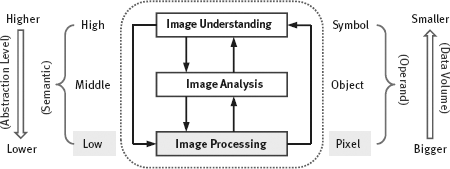
\includegraphics[width=0.8\textwidth, keepaspectratio]{08_Chapter01_fig1-4}
	\caption{\label{fig:sota:imageengineering} Levels of image engineering. 
	Reprinted from \textcite[][Chapter~1]{zhang2017imageprocessing}}
\end{figure}

\subsection{Image Representation}
Image data can be captured with different systems which produce image data of various dimensions.
It consists of information that can be visualized in any manner, such as still picture in color or grey-scale, a video, or a volumetric scan \autocite[][Chap.~1]{zhang2017imageprocessing}.
In general an image can be though of as a function $f: D \rightarrow V$, 
where $D$ is the domain of the location of an point in the image 
and $V$ is the domain of the properties of the real world represented at this point.
Typical examples for $ D $ are two dimensional images where the points are of the form $ (x, y) $, three dimensional images with points of the form $ (x, y, z) \in \mathbb{R}^3 $ or videos with points of the form $ (x, y, t) \in \mathbb{R}^3 $ where $ t $ is the time dimension.
Typical examples for $ V $ are grey-scale images where the luminosity is described as a value in $ \mathbb{R} $ or a colored image where the color is describes as a red-green-blue $ (r, g, b) \in \mathbb{R}^3 $.

For digital images $V$ and $D$ are discrete with upper and lower limits.
In two dimensions a image point a discrete position $ (y, x) \in \mathbb{N}^2 $ is called a \emph{pixel},
in three dimensions a point $ (x, y, z) \in \mathbb{N}^3 $ is called a \emph{voxel}.
In order to store such an image on a computer a \emph{matrix representation} can be chosen.
Examples:
For two dimensional images this matrix is element of $ V^{X \times Y} $, where $ X $ and $ Y $ describe the width and height of the image \autocite[][Chap.~1]{zhang2017imageprocessing}. For three dimension $ V^{X \times Y \times Z} $ can be used, where $X Y Z$ describe the length of the image in each spatial direction. 
A discrete (digital) two dimensional \ac{RGB} color image can be represented as a matrix  $ F \in \mathbb{N}^{X \times Y \times 3} $.
The value of a pixel can then be obtained using the function $ f_F: \mathbb{N}^2 \rightarrow \mathbb{N}^3 ; (x, y) \mapsto f(x,y) = F_{x,y} $.

\subsection{OpenCV Computer Vision Library}
OpenCV (Open Computer Vision Library) is a free (as in freedom) and open-source library,
which collects many common functionalities for advanced computer vision.
The \ac{BSD} license allows it to be used in private, academic and commercial contexts. 
It is written in performant C/C++ and offers \ac{API} bindings for C++, Python and Java on Windows, Linux, Mac OS, iOS and Android \autocite[][]{opencv2018opencv}.
It features algorithms that operate on all three layers of image engineering as defined by Zhang 
and can be used to implement complex visual systems. 
Its documentation is extensive and offers practical examples for a lot of problems it solves.



\subsection{2D Object Detection}

\subsubsection{Convolution Kernels}

A key concept in image processing is the application of an \emph{convolution matrix} to an image, which is also known as a \emph{kernel}. 
It is a small matrix with the same dimensions as the image it is applied to. 
For \ac{2D} images $ 3 \times 3 $ or $5 \times 5 $ kernels are used. 
To apply the kernel to the image, they are convoluted.
This is done for each pixel individually by \enquote{overlaying} the kernel with its center onto it. 
Then the sum of the element-wise multiplication of the kernel and the overlaid area of the image is calculated in order to determine the resulting pixel value in the output image.
For a \ac{2D} image $ F \in \mathbb{N}^{X \times Y} $ the convolution $ H \in \mathbb{N}^{X \times Y} $ using the kernel $ K \in \mathbb{N}^{M_i \times M_j} $ is calculated with the formula in figure \ref{eq:sota:convolution}:

\begin{figure}[h!]
\begin{equation*}
H_{x,y} = \sum_{i=0}^{M_i-1} \sum_{j=0}^{M_j-1} F_{x+1-a_i, x+j-a_j}K_{i,j}
\end{equation*}
\caption{Application of an 2D convolution kernel. Reprinted from the \textcite[][]{opencv2018kernel}}
\label{eq:sota:convolution}
\end{figure}

Convolution kernels can be used to find local features in an image or apply general local operation.
This includes blurring with the Gaussian filter, and edge detection with the Sobel filter in X and Y direction or with the Laplace filter (see figure \ref{eq:sota:kernels}).
It can also be used to sharpen an image. 
The use of convolution kernels is not limited to \ac{2D} images, 
the same method also works for higher dimensional images, 
when appropriate kernel matrices are used.

\begin{figure}[h!]
\begin{equation*}
    G = 
    \dfrac{1}{16}
    \begin{bmatrix}
    1 & 2 & 1 \\
    2 & 4 & 2 \\
    1 & 2 & 1
    \end{bmatrix}
    ;
    G_x = 
    \begin{bmatrix}
    1 & 0 & -1 \\
    2 & 0 & -2 \\
    1 & 0 & -1
    \end{bmatrix}
    ;
    G_y = 
    \begin{bmatrix}
    1 & 2 & 1 \\
    0 & 0 & 0 \\
    -1 & -2 & -1
    \end{bmatrix}
    ;
    D_{xy}^{2} = 
    \begin{bmatrix}
    1 & 1 & 1 \\
    1 & -8 & 1 \\
    1 & 1 & 1
    \end{bmatrix}
\end{equation*}
\caption{Examples for kernels left to rigth: Gaussian blur filter, Sobel filter in X direction, Sobel filter in Y direction, Laplace filter}
\label{eq:sota:kernels}
\end{figure}

\subsubsection{Background Subtraction}
Background subtraction used to detect areas of interest in a video.
Especially in a static camera setup, everything that moves can be considered the foreground and everything that stays static is the background. 
To do so, a model of the background without any moving objects is needed.
It acts as a reference frame to compare the current frame of a video against.

If an image is available, that only shows the background of a scene,
\emph{static background subtraction} can be used.
In this method, the current frame of the video and the background are blurred 
and the element-wise absolute difference between the images is calculated.
If the absolute difference for a pixel is higher than a specified threshold, then the pixel is considered part of the foreground.
This method uses the given background image as a static model for the background and does not update the model if the background changes.

When no pure background image is available 
or if the background can change over time, e.g. by different lighting,
the background model needs to be regularly adapted.
\textcite[][]{piccardi2004background} presents an overview of techniques used to create such a model, 
whereas here only a subset is presented:

\begin{itemize}
    
    \item \textbf{Running Gaussian average} For each pixel $ I $  in the grey-scale video image a running average $ \mu{}_t$ is calculated, that is updated in each frame by the formula $ \mu{}_t = \alpha{}I_t + (1 - \alpha)\mu{}_{t-1} $, where $ \alpha $ is an weight that determines how fast the model is updated. The variance $ \sigma{}_t $ is calculated similarly. A pixel $ I_t $ is considered foreground if $ |I_t - \mu{}_t| > k\sigma{}_t $ holds, where $ k $ is a parameter that determines the threshold sensitivity of the algorithm.
    \item \textbf{Mixture of Gaussians} Instead of assuming a single value likelihood distribution for each pixel, multiple Gaussian distributions are used in this method introduced \textcite[][]{stauffer1999background}. 
    When using $ K $ distributions this enables the distinction of $ K $ types of background and foreground, which improves the detection rate in outdoor scenes where e.g. leafs and branches of trees might be present. 
    For each of the $ K $ distributions the peak amplitude $ \omega{}_{i,t} $, average $ \mu{}_{i,t} $ and variance $ \sigma{}_{i,t} $ are stored.
    The distributions are ranked by the ratio $ \omega{}_{i,t} / \sigma{}_{i, t}$, since more narrow distributions are assumed to belong to a background classification.
    The distributions are checked in order of their rank to accept a pixel value when $ (I_t - \mu{}_{i,t})/\sigma{}_{i,t} > 2.5 $ holds, where $ I_t $ is the current pixel value.
    If $ \omega{}_{t} $ of the first accepting distribution is higher than a threshold, the pixel is considered background.
    The distribution parameters are updated using a running calculation (as above) when a new pixel value is a accepted by it.
    If no distribution accepts the value, the distribution with the lowest ranked is replaced by a new distribution centered around the new value with a high variance.
    Improved forms of this algorithm exist, like \autocite[][]{chan2011background}, and are currently used.
    
\end{itemize}

Since video images can contain pixel level noise, it is useful convert color video to grey-scale and to blur the images before applying the background subtraction.

\subsubsection{Blob Detection}

A \emph{blob} in a binary mask image is an area that consists of 

what is a blob

first explain contour (what are contours: outlines of connected areas in a binary mask) detection by border following \autocite[][]{suzuki1985border}



\autocite[][]{opencv2018blob}
operates on binary masked image
\begin{enumerate}
    \item Find the contours present in the image and calculate their centers
    \item Group these centers based on a threshold for the distance for their location
    \item From these groups, find overall center and estimate area and radius of the blob
\end{enumerate}

TODO

\subsubsection{Convex Hull}

TODO
edge detection, outline detection, silouettes, contours
foreground background mask from video image
background substraction
convex hull


\subsection{3D Volume Estimation}

TODO describe what is ment by this

\subsubsection{Camera Projection and Calibration}

Since camera lenses use a perspective projection to produce images, 
there are several considerations needed when working with \ac{3D} scenes that are captured.
The points in the 3D scene can be described as coordinates in the \emph{world space}.
In the perspective projection these points are seen from a single point in the camera, 
which is the sensor in a real camera.
To perform the projection the position of the point seen on the \emph{image plane} is calculated.
The image plane is the section of the scene that is seen by the camera in the distance of the focal length.
Figure \ref{fig:sota:camerprojection} shows how this projection can be visualized.
Note that the Z axis is pointing into the real world space in the direction the camera is looking to.
Since this projection is dependent on the focal length of the camera and the principal point, which is seen in the center of the image, it can be described as the intrinsic camera matrix $ A $ in the equation in figure \ref{eq:sota:camcalib}.
When world space and camera space coordinates are not the same, i.e. the camera is rotated or translated, there exists an additional rotation and translation matrix $ [R|t] $ that describes these external projection parameters.

\begin{figure}[hbt]
    \centering
    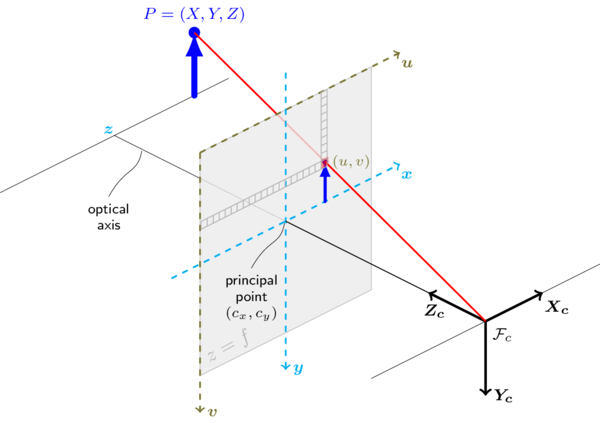
\includegraphics[width=0.8\textwidth, keepaspectratio]{opencv_pinhole_camera_model}
        \caption{Camera model to illustrate perspective projection of a 3D scene onto the image plane (grey). Reprinted from the \textcite{opencv2018calibration}}
    \label{fig:sota:camerprojection}
\end{figure}

\begin{figure}[h!]
\centering
\begin{equation*}
    s m' = A[R|t]M'
    \hspace{2em}
    \Longleftrightarrow{}
    \hspace{2em}
    s 
    \begin{bmatrix}
        u \\
        v \\
        1
    \end{bmatrix}
    =
    \begin{bmatrix}
        f_x & 0 & c_x \\
        0 & f_y & c_y \\
        0 & 0 & 1
    \end{bmatrix}
    \begin{bmatrix}
        r_{11} & r_{12} & r_{13} & t_1 \\
        r_{21} & r_{22} & r_{23} & t_2 \\
        r_{31} & r_{32} & r_{33} & t_3
    \end{bmatrix}
    \begin{bmatrix}
        X \\
        Y \\
        Z \\
        1
    \end{bmatrix}
\end{equation*}
\caption{Camera calibration with internal and external parameters. Reprinted from the \textcite{opencv2018calibration}}
\label{eq:sota:camcalib}
\end{figure}

The equation in figure \ref{eq:sota:camcalib} depicts how a point in the world coordinate system can be mapped to the image plane of a camera. 
The following list explains the mentioned coefficients:

\begin{samepage}
\begin{itemize}
    \item $ s $ is the scale factor for image, such that the z axis of the image plane is 1
    \item $ (X, Y, Z) $ is the 3D point in world space
    \item $ (u,v) $ is the projected point in the image plane
    \item $ A $ is the internal camera matrix
    \item $ (c_x, c_y) $ is the principle point in the world space seen at the image center
    \item $ f_x, f_y $ are the focal lengths in pixel units
    \item $ R $ is the external rotation matrix
    \item $ t $ is the external translation vector
\end{itemize}
\end{samepage}

The internal camera matrix $ A $ can be calculated from multiple images of an object with known structure and dimensions, called a \emph{calibration pattern} \textcite{opencv2018calibration}. 
For example an chessboard can be used, which is photographed from different positions and angles. 
The corners of the chessboard squares are used determine how a straight line is projected in the camera in order to approximate the internal camera matrix.

The external parameter for rotation and translation can not be found from one camera alone.
In a multi-camera setup they can be found by triangulation of multiple points in multiple images that show the same scene from different angles.
If this triangulation is not possible because the points used for triangulation are not visible from all camera perspective, the rotation matrix an the translation vector can be found out by measuring the real world.
The rotation matrix can be calculated by measuring the relative rotation angles of the cameras to each other.
The equation in figure \ref{eq:sota:rotation} can be used to determine the combined rotation matrix when the rotation around the yaw, pitch and roll angles are known. 
Yaw pitch and roll describe the rotation around the Z, Y and X axis respectively.
The translation vector can be found by measuring the distance of the cameras to each other.

\begin{figure}[h!]
\centering
\begin{equation*}
    R
    =
    R_z(\alpha)R_y(\beta)R_x(\gamma)
    =
    \begin{bmatrix}
    cos \alpha{} & - sin \alpha{} & 0 \\
    sin \alpha{} & cos \alpha{} & 0 \\
    0 & 0 & 1 
    \end{bmatrix}
    \begin{bmatrix}
    cos \beta{} & 0 & sin \beta{} \\
    0 & 1 & 0 \\
    - sin \beta{} & 0 & cos \beta{}
    \end{bmatrix}
    \begin{bmatrix}
    1 & 0 & 0 \\
    0 & cos \gamma{} & - sin \gamma{} \\
    0 & sin \gamma{} & cos \gamma{} 
    \end{bmatrix}
\end{equation*}
\caption{External rotation matrix from rotation along the yaw, pitch and roll angles $ \alpha{} $ , $ \beta{} $ and $ \gamma{} $ }
\label{eq:sota:rotation}
\end{figure}

Furthermore real lenses introduce optical aberrations and 
there exists \emph{distortion} in camera images.
Distortion is visible in the effect where straight lines appear curved in the image representation.
There exists two kinds of distortion that can occur, namely radial and tangential distortion \autocite[][Fig.~2]{weng1992distortion}.
Radial distortion makes points appear closer together or further apart depending on their distance to the image center. 
It is visible as a \enquote{barrel} or \enquote{pillow} effect on rectangular lines. 
Tangential distortion causes a rotation of the image depending on the distance and angle of a point to the image center.
The amount and type of distortion is part of the internal camera parameters.
Just as the matrix of intrinsic parameters, the parameters for the distortion can be calculated from images of structures with known dimensions
\autocite{opencv2018calibration}.

\subsubsection{Single View Estimation}
When the geometric shape of an \ac{3D} object is roughly known beforehand and only its exact outline and scale varies, it is possible to estimate its volume from its outline in a single image.
The assumption here is that the volume scales with the area, that the object covers on the image \autocite{levine1989microwave} \autocite[][]{wang2017apple} \autocite[][]{sapkal2017volume} .
Therefore a reference object with known dimensions is necessary to calculate the scale against.
This approach avoids the need to multiple cameras and a \ac{3D} calibration
However it does not generalize to \ac{3D} objects of unknown shape.

\subsubsection{Feature Based Scene Reconstruction} 
stereo vision
of full \ac{3D} reconstruction of each point
TODO

key concept: photoconsistency : a voxel is photoconsitent when 



\begin{figure}[hbt]
	\centering
	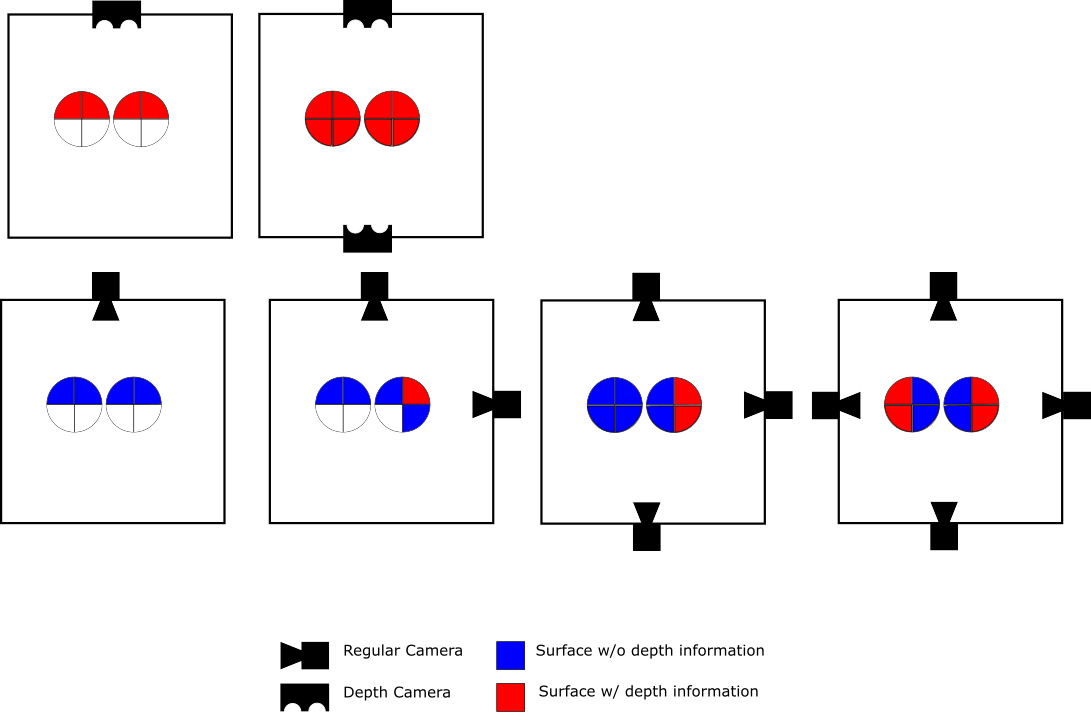
\includegraphics[width=1.0\textwidth, keepaspectratio]{resources/multiview}
	\caption{\label{fig:sota:mulitviewtop}Concept of depth reconstruction in a 2D multi-view situation.
	Adapted from \textcite[][]{sonaten2011volume}}
\end{figure}

\subsubsection{Silhouette Based Volume Reconstruction}

The \emph{silhouette} of an object within an image is intuitively defined 
as a binary mask describing the areas of the image in which the object is present. 
The edges of this areas describe the contours of the object.
The silhouette can be obtained by image segmentation of the original image \autocite[][Chap.~2]{zhang2017imageanalysis}, such as by background substraction.
Depending on the camera perspective different portions of the object are visible.
Only the outline of the object from this perspective is visible.
This implies that is is not possible to capture concave parts of an object.

Silhouettes from multiple perspectives can be used to reconstruct the \ac{3D} shape of an object from \ac{2D} images of said object.
The reconstructed \ac{3D} shape does not represent the real geometry of the object, but produces the same silhouettes as the real object when seen from the angles it was reconstructed from.
The shape that is constructed from the silhouettes is called \emph{visual hull}, a term introduced by \textcite[][]{laurentini1994hull}.
Since the silhouette does not include information about concavities,
the visual hull also is convex. 
Furthermore the silhouette does not include information about parts of the object whose visibility is obstructed from a certain perspective.
Therefore the visual hull can not describe the shape of  part of the object, that are not visible in any silhouette.

\begin{figure}[hbt]
	\centering
	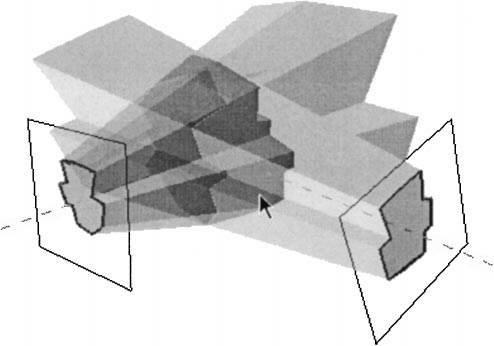
\includegraphics[width=0.6\textwidth, keepaspectratio]{resources/volume_intersection_bottino}
	\caption{\label{fig:sota:volumeintersection} Volume intersection of cones from silhouettes.
	Reprinted from \textcite[][]{bottino2001silhouette}}
\end{figure}

Figure \ref{fig:sota:volumeintersection} visualizes how the visual hull is created from two silhouettes. 
Since the cameras that capture the silhouette are perspective,
cones are used for the projection of it into the object space.
The intersection of those cones creates the visual hull.
There are several methods to implement silhouette based shape reconstruction:

\begin{itemize}
    \item \textbf{Standard Voxel Based Method} 
    In this method, first the space too be modeled is described as a \ac{3D} grid of voxels at an constant resolution.
    To find out which voxels belong to recontructed object,
    each voxel is projected into the viewport of each camera 
    and it is checked whether it lies in the silhouette from this perspective.
    Only if it lies inside of all silhouettes
    it remains part of the finale volume description.
    \item \textbf{Space Carving}
    Space Carving (substractive technique that begins with a full voxel scene. the surface oof the scene is carved away pixel per pixel untill all surface voxels  are photoconsistent, this also provides the possibility to determine the color of the shape)
\autocite[][]{kutulakos1999spacecarving}
\end{itemize}

TODO still needs a reference or calibration to determine the space of the modeled room / scaling factor

TODO
multiview, depth sensors
interpolation of depth information by combinding views
bounding / section box
convex hull in 3d by mask


\section{Elevator Control}

When looking at elevator systems that are installed in buildings
one property that is noticeable to the passenger, except for the physical properties, is the way the elevators are moved in order to pick up and deliver the passengers to their destination.
The algorithms used to control this movement influence how long the passenger needs to wait for a cabin and how long their journey takes.
Therefore it affects the perceived quality of the system.
However in buildings with an increased traffic demand, it is necessary to use elevator systems with multiple cabins and more complex control strategies.
In this section the general principles about those control strategies are laid out.

\subsection{System Components}

In order to gain an understanding of how an elevator system is controlled,
it is useful to look at the components a general system includes.
To do so, the mechanisms involved in a typical elevator ride 
from a passenger perspective shall be outlined.
Figure \ref{fig:sota:systemcomponents} gives an general overview over the involved logical components and their connections.

\begin{figure}[hbt]
	\centering
	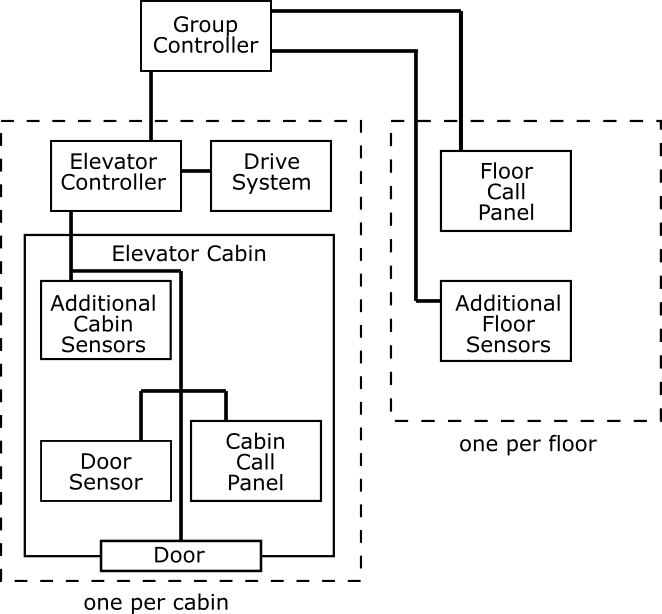
\includegraphics[width=0.8\textwidth, keepaspectratio]{resources/systemcomponets}
	\caption{\label{fig:sota:systemcomponents} General components of an elevator control system. Adapted from \textcite[][pp.~4,16]{xang2016trafficlist} and  \textcite[][p.~10]{siikonen1997models}}
\end{figure}

When a passenger wants to take the elevator from one floor to another,
they press a button on the \emph{floor call panel} and issue a \emph{hall call} (or \emph{reservation call}, \emph{landing call}) to the system \autocite[][pp.~6--10]{siikonen1997models}.
This hall call signals to the system that an elevator needs to pick them up.
The button pressed might be a simple push button, but can also be more complex 
and capture information about the direction or destination of travel \autocite[][pp.~89--93]{unger2015aufzuege}.
Even before the passenger presses the panel button, \emph{additional sensors} 
on the floor can detect their intent to use the elevator and gather more information about them.
This can include among others camera systems \autocite[][]{lin2011control}, badge scanners, or \enquote{smart home} installations \autocite[][]{kwon2014sensor}.
In a multi-elevator system the hall call is registered by the \emph{group controller} and stays active until it is deleted when an cabin picks up the passenger.
The group controller \emph{schedules and dispatches} an elevator move to the respective floor and serve the call.
In case of a single-elevator system no group controller is necessary.
Different scheduling algorithms can be used to determine which cabin should serve which hall call next.
The dispatch signal is picked up by the \emph{elevator controller} of the respective cabin, which then instructs the \emph{drive} system to move the elevator along the shaft to the respective floor by actuating the motors.

Once a cabin stops at the floor, it opens its \emph{door} and the passenger enter the elevator.
To select their destination floor, they use the \emph{cabin call panel}.
This \emph{car call} (or \emph{destination call}) \autocite[][pp.~6--10]{siikonen1997models} is passed to the group controller, 
which schedules the elevator to move to the destination floor at some time.
The group controller needs therefore to consider hall calls, as well as car calls in its scheduling algorithm
Before the elevator starts to move, the door closes again, if no obstacle is detected by the \emph{door sensor}.
Until the elevator serves the destination floor, the car call stays active.
\emph{Additional sensors} inside the cabin provide more information about the passengers inside.
This can include among others a weight scale to measure the total weight utilization, or a kind of camera system \autocite[][]{xang2016trafficlist}.
Further more the position of each elevator is known to the group controller.

\subsection{System Classifications}

Elevator systems come in different configurations with different purposes.
Depending on their use cases different technical implementations can chosen.
Therefore they can be classified in various dimensions.

The first observation to make is the \textbf{number of shafts and cabins} in the system.
The main difference comes in the scheduling complexity regarding single-cabin versus multi-cabin systems.
Systems with multiple elevators need a group controller to decide which cabin serves which hall call.
This decision can be non-trivial as laid out in section \vref{sec:sota:strategies}.
When only one cabin is used, the scheduling becomes more straightforward.
In small residential buildings an single cabin might be sufficient.
However in buildings with larger passenger amounts, such as office buildings, a multi-elevator setup can become necessary increase the handling capacity.

Next is the classification by the \textbf{type of objects or people} that are transported in the system. Especially important is the distinction of the purpose of the elevator system regarding whether people and / or large objects can be conveyed.
\textcite[][pp.~141--158]{unger2015aufzuege} describes the properties of the most common types:

\begin{itemize}
    \item Cabins that carry \textbf{only people} 
    typically have a premium interior decoration, such as glass, mirrors or stainless steel.
    Usually also cargo can be transported, but large goods might damage the cabin.
    Examples for a building that uses such elevators are office buildings, residential buildings or hotels.
    
    \item Elevators for \textbf{large cargo and people} 
    have a more simple interior that is more resistant to damage by lifting carts. 
    However security measures regarding the doors are taken, such that the elevator is also safe to use by people. 
    Typically a high payload weight and dimension can be moved.
    Examples for the usage of this type are factories, storage buildings or hospitals. 
    
    \item Lifts that carry \textbf{only small cargo} can be found for example in restaurant kitchens to transport dishes.
    The cabin is not used by people and the system is controlled purely from outside call panels. 
    Due to the size restriction only a smaller weight needs to be transported.
    
    \item Cabins that convey \textbf{only large cargo} but no people can only be controlled from the outside call panel and have fewer safety restrictions, even though the cabin can be entered for loading and unloading. 
\end{itemize}

This excerpt of the list is far from complete and \textcite[][pp.~141--158]{unger2015aufzuege} lists even more types, 
such as lifts for wheel chairs, the never-stopping paternoster or elevators on construction sites.
However these are not in the scope of this thesis and are not further considered.

Another interesting distinction to consider is the \textbf{amount of floors} that is served by an elevator system.
The amount of floors influences the heeded handling capacity of the system.
The more floors there are, the more people need to travel a potentially longer distance.
While a building with only a few floors can be handled by a single elevator,
buildings with up to 40 stories require the use of elevator groups.
When more than 40 floors need to be served, 
introducing a \emph{sky lobby} can be beneficial, 
where a fast shuttle transports passengers between the main lobby and the sky lobby. Passengers can then switch the elevator to reach their final destination \autocite[][p.~9]{hakonen2003simulation}.

%
%TODO
%- by type of sensory to haul the car
%-- single button
%-- direction button
%-- destination control
%-- camera system

%TODO additional travel information: how many people inside and outside, up / down / floor %select inside / outside, everyone presses?, video? 
%destination control system


\subsection{Passenger Traffic Patterns}
Passenger traffic patterns are typical streams of passengers going from one floor to another.
Those patterns are reoccurring regularly based on the time of the day.
The movement of passengers can be described with three directions: \emph{incoming}, \emph{outgoing}, and \emph{inter-floor} traffic.
With those directions the traffic patterns can be described, as they focus on one of the directions, but also incorporates components of passengers heading in other directions \autocite[][p.~259]{siikonen1993simulation}.
According to multiple sources, three general patterns are present in office buildings \autocite[][pp.~1--2]{beers2015arrivals}
\autocite[][pp.~6--7]{axelsson2013strategies}
\autocite[][p.~194]{unger2015aufzuege}
\autocite[][p.~14]{siikonen1997models}:

\begin{itemize}
    \item \textbf{Up-peak traffic} In the morning the majority of passengers in an office building constitutes to an incoming traffic.
    They arrive at the entrance lobby and travel to different upper floors to fill the building.
    The lift cars potentially need to stop at every level and return to the lobby without passengers to pick up new ones. 
    This reduces the utilized capacity and puts a high load on the elevator system to convoy all passengers in time.
    \item \textbf{Down-peak traffic} In the evening the majority of the passengers are leaving the office building and travel from arbitrary upper floors to the main lobby.
    Most of the passengers constitute to outgoing traffic.
    The elevator system needs to pick up passengers at every level. 
    Reverse to the up-peak traffic, the cars are empty when returning from the lobby.
    Similar to the up-peak traffic this situation induces a high stress on the system.
    \item \textbf{Inter-floor traffic} All other traffic that is neither incoming nor outgoing can be considered inter-floor traffic. Passengers that travel from one floor to another but are not entering or leaving the building are the majority in this situation.
\end{itemize}

\begin{figure}[hbt]
	\centering
	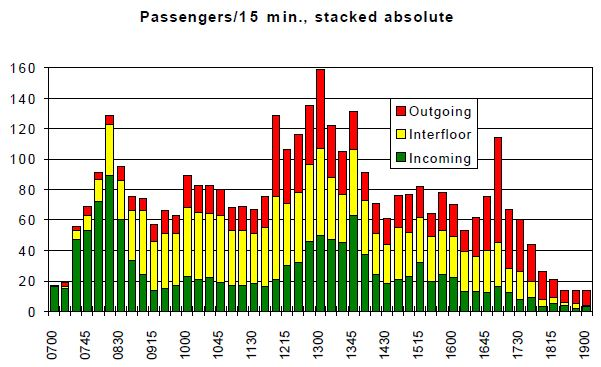
\includegraphics[width=0.8\textwidth, keepaspectratio]{resources/traffictimes}
	\caption{\label{fig:sota:traffictimes} Exemplary traffic component profile for an office building.
	Reprinted from \textcite[][p.~14]{siikonen1997models}}
\end{figure}

%Figure \ref{fig:sota:trafficpatterns} depicts the former mentioned traffic components.
Figure \ref{fig:sota:traffictimes} shows an example of how the traffic components contribute to overall traffic in an office building. A clear peak of incoming traffic in the morning and outgoing traffic in the evening are visible.
This information can be used to model simulations and predict traffic in various circumstances.
It has significant impact on the scheduling principles employed for each situation in order to improve the efficiency of an elevator system.

%\begin{figure}[hbt]
%	\centering
%	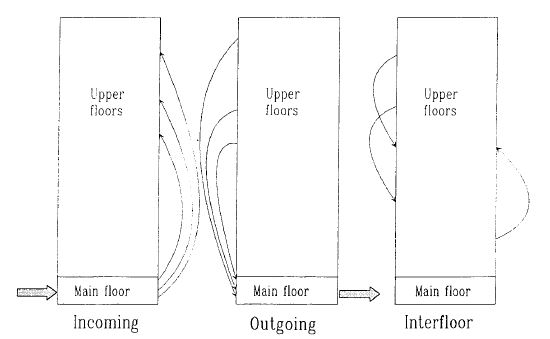
\includegraphics[width=0.8\textwidth, keepaspectratio]{resources/trafficpatterns}
%	\caption[]{\label{fig:sota:trafficpatterns} Typical categories of passenger traffic: Incoming, Outgoing and Inter-floor.
%	Reprinted from \textcite[][p.~259]{siikonen1993simulation}}
%\end{figure}

% TODO or use \textcite[][p.~12]{sorsa2005destination} as broader image 

\subsection{Control Strategies}
\label{sec:sota:strategies}

Elevator control strategies deal with the assignment of hall calls and car calls to elevator rides in order to derive a stopping schedule for the cabins in the system.
The way this schedule is set up affects
the performances regarding the criteria laid out in section \label{sota:sec:perf}.
An appropriate control algorithm must be chosen in order to optimize for performance criteria
depending on the type of elevator system, it's use purpose and the current passenger traffic.
Depending on the type of elevator system different control strategies are used, some of which are listed below.

\subsubsection{Sequential Control}
In contrast to the strategies below, 
this strategy is only applicable to a single-lift system.
The system answers hall calls in the order they arrive 
and executes the car call with priority before moving on to serve the next hall call.
This way only one ride is performed a time and the calls are executed in sequence. This method is also called \emph{single call automatic control} or \emph{non-collective control}.
Drawbacks of this strategy are a increased passenger waiting time and an decreased handling capacity.
However for cargo lifts, this can beneficial if only on cargo item can fit the cabin at a time
\autocite[][p.~238]{barney2016handbook}.

\subsubsection{Collective Control}
This is the \enquote{most common form of automatic control} \autocite[][p.~237]{barney2016handbook}.
Hall calls are answered in the order of the floors they originate from rather than their temporal order.
On the way up and down the cabin collects all the hall calls and deliver car calls also following the floor order.
Different variations of this approach are available, where the direction of the hall call is ignored, only downward calls are collected only upwards calls are collected, or the call direction is considered for collection in both directions.
This approach can be expended to a elevator system with group control, such that a hall call is answered by the first cabin to pass the floor in the desired direction \autocite[][p.~238]{barney2016handbook}.
When all cabins are idle, the nearest available is assigned to a call. Hence this strategy is also called \emph{nearest car}
\autocite[][p.~244]{barney2016handbook}.

\subsubsection{Zone Approach}
In this approach the floors of the building are divided into static, continuous zones also called \emph{sectors} \autocite[][p.~247]{barney2016handbook}. 
Typically there are is one zone per elevator in the group. 
Each lift in the group serves hall calls from only one sector
while also delivering passengers to floors outside of this zone
\autocite[][pp.~3--6]{axelsson2013strategies}.
The order of serving of the hall calls is based on the collective control.
A lift is currently outside of its zone, 
the zone can be served by lifts from sectors above and below it.

The distribution of zones can be chosen based by the amount of passengers on each floor.
This approach is useful when the traffic is evenly distributed across the building, such as in interfloor traffic. It can be complemented with controls for special condition to react to peak-traffic \autocite[][p.~247]{barney2016handbook}.
The static zone approach can be extended to a dynamic sector approach where the sectors are not limited by static floor numbers but by the position of the elevators \autocite[][p.~250]{barney2016handbook}.

\subsubsection{Cost-function based approches}

\subsubsection{Parking Policies}

TODO
single elevator  vs multi elevator
TODO: more types

\autocite[][pp.~3--4,10]{beers2015arrivals}
- parking polcies
- call allocation

\autocite[][pp.~3--6]{axelsson2013strategies}
- search based
- rule based
- genetic algorithm




\subsection{Performance Criteria}
\label{sota:sec:perf}

In order to evaluate the performance of an elevator system some metrics about it are commonly considered.
They are used to check if a planned system fulfills the requirements that the expected traffic poses. 
The metrics are mostly perceived as part of the service quality by the passengers.
Many of them are linked together and influence each other.

% General cite:
%\autocite[][p.~10]{beers2015arrivals}
%\autocite[][p.~7]{hakonen2003simulation}
%\autocite[][pp.8-9]{siikonen1997models}
%\autocite[][p.~194]{unger2015aufzuege}

\begin{itemize}

    \item The \textbf{passenger waiting time} 
        describes the amount of time between the arrival of a passenger at the landing floor 
        and their entry into the elevator cabin 
        \autocite[][p.~7]{hakonen2003simulation}\autocite[][pp.8-9]{siikonen1997models}.
        
    \item The \textbf{passenger ride time} 
        measures the time between the entering of a passenger into the cabin 
        and them exiting the cabin on the destination floor
    \autocite[][pp.8-9]{siikonen1997models}.
    
    \item The \textbf{total journey time}, 
        also called \emph{total service time} \autocite[][p.~10]{beers2015arrivals} or \emph{time to destination},
        describes the total time a passenger spends in the system 
        and is calculated by the sum of waiting and ride time
        \autocite[][pp.8-9]{siikonen1997models}.
        
    \item The \textbf{round trip time} 
        describes the time it takes for a single elevator to collect passengers at the lobby,
        deliver them to the upper floors and return to the lobby. 
        This measure is critical in the up-peak traffic
        \autocite[][pp.8-9]{siikonen1997models}.
        
    \item The \textbf{handling capacity}, 
        also called \emph{5-minute interval}
        \autocite[][p.~194]{unger2015aufzuege},
        describes the maximum number of passengers that can be transported (into the upper most floor) during up-peak traffic
        \autocite[][pp.8-9]{siikonen1997models}.
        It is dependent on the round trip time.
        In theoretical considerations a maximum utilization of 60-80\% of the capacity is used for this scenario
        \autocite[][p.~194]{unger2015aufzuege}\autocite[][p.~7]{hakonen2003simulation}.
    
    \item The \textbf{interval time} 
        describes the time between departures of any cabin from the lobby 
        and influences the time a passenger hat to wait at the lobby
        \autocite[][pp.8-9]{siikonen1997models}.
    
    \item The \textbf{hall call time} 
        describes the time between the issuing of an hall call by a passenger and the cancellation of the call. 
        The call is canceled when an elevator is scheduled to serve the call floor and hence decelerates to stop at the floor
        \autocite[][pp.8-9]{siikonen1997models}. 
    
    \item The number of \textbf{total stops}
        necessary to serve an specified amount of passengers (or within a given time frame) is an indicator for the efficiency of the scheduling algorithm
        \autocite[][p.~194]{unger2015aufzuege}.
    
    \item The \textbf{energy consumption} 
        per ride or per time interval is an measure of economic interest. 
        However it does not influence the perceived service quality.
    
    \item The \textbf{capacity utilization} 
        of the cabins in spacial and weight dimensions is an interesting metric to observe, 
        since usually only 60-80\% of the capacity is used at a time 
        \autocite[][p.~194]{unger2015aufzuege}
        \autocite[][p.~7]{hakonen2003simulation}.
        This utilization can be even lower when large objects are present.
        The average utilization is further influenced by empty rides.
        
\end{itemize}

For each of the metrics it is common to calculate statistical figures, such as average, mean, minimum, maximum and standard deviation, which also can differ depending on the traffic situation.
These calculations can be based on theoretical consideration about the physical parameters of the system \autocite[][p.~194]{unger2015aufzuege}, simulations or heuristical observations in real buildings.
 
When the group controller schedules the elevators in a system, the order of dispatches influences the metrics listed above.
The elevator allocations are calculated by optimization of a cost function which takes the metrics in consideration.
Usually the waiting time is optimized, but also the ride time can be optimized in order to increase the handling capacity. \autocite[][p.~10]{siikonen1997models} 

\subsection{Optimization Approaches by Simulation}
TODO
model building etc: here is a lot of research in the topic utilizing theoretical multivariable model optimization, simulational approaches and heuristical approaches in real world (refs?)

\autocite[][pp.~7--11]{beers2015arrivals}
\autocite[][p.~193]{unger2015aufzuege}


TODO

% !TEX root = ../master.tex
\chapter{Design and Methodology}
\label{chap:design}
This chapter describes which research method is used to design a solution 
that answers the initial questions posed in the first chapter.
The considerations that contribute to the design of this solution are outlined 
and form the foundation for its implementation in the next chapter.

\section{Employed Methodology}

Preceding to the practical part of this thesis, 
the method to follow along shall be laid out here.
One suitable method is the general concept of \emph{design science research}, also known as \emph{constructive research}, 
since it involves the development and evaluation of artifacts to solve domain specific problems.
It therefore conveys a improved practical relevance in comparison to purely descriptive research methods,
while the outcomes still create scientific knowledge
\autocite[][p.~v]{dresh2015designresearch}.
The conducted research must design an artifact, such as a construct, model or method, that solves a relevant problem in a specific field, which is evaluated regarding its utility, quality and efficacy.
The performed research should be based on rigorous scientific methods and contribute to the current theoretical body of knowledge.
The conducted design process must take into account the practical environment it is executed in and use the available resources.
A conclusion of the project for both technology-oriented as well as management-oriented audiences should be presented in the end
\autocite[][p.~70]{dresh2015designresearch}.

\begin{figure}[hbt]
	\centering
	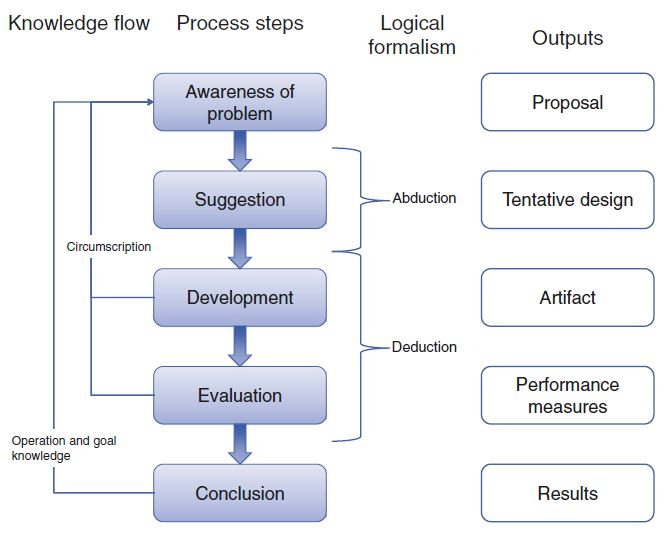
\includegraphics[width=0.8\textwidth, keepaspectratio]{resources/designscienceresearchoutputs.jpg}
	\caption{\label{fig:design:designscience} Process steps and outputs of design science research. Reprinted from \textcite[][p.~83]{dresh2015designresearch}}
\end{figure}

Figure \ref{fig:design:designscience} displays the steps that are found in the process of design science research. 
Those are the steps that guide the execution of this thesis.
The awareness and relevance for the given problem has already been given in section \vref{sec:into:context}.
Looking back to the original research questions (see section \vref{sec:intro:goals}) two focuses have been identified for this thesis:

\begin{itemize}
    \item Which computer vision techniques can be used to detect persons and objects within an elevator car and in front of the lift and estimate their spacial volume?
    \item How can the information acquired by a system that uses such methods constitute to the optimization of algorithms that control the movement plan for elevators?
\end{itemize}


To answer the two questions, the conducted research is therefore twofold.
The first part involves the design and experimental implementation of a system to gather passengers volume data in elevators.
The second part deals with the integration of this information into a scheduling algorithm.
Outlined below are the steps that are taken to
suggest a tentative design for each, develop the artifacts and evaluate them.

For the  design and implementation of a vision system to gather volume data of passengers,
the following steps are performed:

\begin{enumerate}
    \item Find a typical or actual elevator control system architecture and define the positions to integrate the necessary components for an vision system into it.
    \item Define the exact type and structure of the information that the vision system should be able to detect.
    \item Find an algorithmic approach to  passenger detection and volume estimation that is suitable to generate the required data.
    \item Match the approach with an possible hardware setup to perform tests with it.
    \item Test the proposed detection system in an real world experiment that includes  exemplary footage from within an cabin and of a lobby.
    \item Evaluate the results of the test for the functionality and effectiveness of the employed system.
\end{enumerate}

For the integration of the  passenger data into existing scheduling algorithm the following steps are performed:

\begin{enumerate}
    \item Define a suitable elevator configuration that could possibly benefit from the information that the vision system can provide. 
    Find a typical or actual control algorithm that is used for such a configuration.
    \item Adapt the scheduling algorithm to use the additional information.
    \item Compare the two versions of the algorithm in order to determine their effectiveness regarding a suitable metric.
    A simulation is used to perform this comparison.
\end{enumerate}

%\begin{figure}[hbt]
%	\centering
%	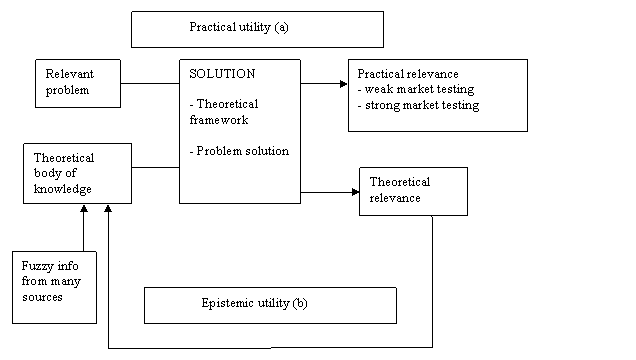
\includegraphics[width=1.0\textwidth, keepaspectratio]{resources/Rasvan_constructive_research_diagram}
%	\caption{\label{fig:design:constructiveresearch} Elements of constructive research. Source:
%	\url{https://en.wikipedia.org/wiki/File:Rasvan_constructive_research_diagram.gif}}
%\end{figure}
 
\section{Visual System}
TODO
\subsection{Proposal for Integration into Elevator Control System Architecture}
TODO
for hardware setup
- no additional sensory
- add cv system (computer) and multiple cams inside each cabin
- add cv system (computer) and multiple or one cam outside on each floor
\subsection{Output Data Definition}
TODO
- for each objects weather it is a person or an cargo object
- for each persons a volume description approximated by an inner and outer ellipse (or simple: circle) as the ground area and a height
- for the cargo objects an approximation as a ground area and a height, possible area types: convex hull most outer circumfence projected to the ground OR estimation by surrounding rectangle
- total number of passengers and cargo objects inside and in-front
\subsection{Detection Technique}
1. Background substraction  to create forground mask
2. space carving to generate voxel representation from different views
3. find distinct items in voxelspace and classify as human or other

\begin{figure}
    \centering
    \tikzset{
      box/.style    = {draw, rectangle, minimum height = 2.5em, minimum width = 2.5em},
      circl/.style  = {draw, circle,minimum size = 8mm},
      input/.style  = {coordinate},
      output/.style = {coordinate},
       to/.style    = {->,>=stealth',shorten >=1pt,semithick,font=\sffamily\footnotesize}
    }
    \begin{tikzpicture}
        
    \end{tikzpicture}
    \caption{Volume detection technique}
    \label{fig:design:volumedetection}
\end{figure}

TODO
\subsection{Test Arrangement and Validation Strategy}
TODO

\section{Scheduling Algorithm}
TODO
\subsection{Suitable Elevator Configuration}
Since the camera system is suitable to detect passengers as well as cargo objects,
it seems reasonable to apply the passenger information 
to a scheduling algorithm of an elevator system which conveys both of them.
This hold the opportunity to have a bigger impact the performance of the system, 
in contrast to applying it to a passenger-only lift.

Looking back at the categorization of elevators, cargo lifts meet this specification.
Typically an office building has one or multiple cargo lifts depending on its size,
but grouping them is uncommon \autocite[][p.~167]{barney2016handbook}.
A weight capacity of at least 1,600 kg is typical \autocite[][p.~167]{barney2016handbook},
but also capacities of 5,000 kg are possible \autocite[][]{kone2017overview}.
Typical application areas for cargo lifts are hospitals, where patients and beds are moved,
auxiliary lifts in office buildings and multi-story industrial buildings.
The typical control algorithm is collective control or sequential control \autocite[][pp.~238,~244]{barney2016handbook}.
For this comparison the sequential control will be taken as a baseline.

\subsection{Adaption of Scheduling Algorithm}
TODO
- when no large cargo is there: collective control
- when large cargo is there: sequential control
- consideration: what to do to switch between collective and seqential control?
\subsection{Preparation for Simulation and Validation Strategy}

TODO simulation configuration:
\autocite[][p.~347]{barney2016handbook}

\begin{table}[]
\centering
\begin{tabular}{lrl}
\textbf{Description} \hspace{5cm}   & \multicolumn{1}{l}{\textbf{Value}}   & \textbf{Unit}   \\
\hline
\multicolumn{3}{l}{\textbf{Building data}} \\
Number of floors & 8 &        \\
Interfloor distances & 3.5 & $m$\\
%& & \\
\hline
\multicolumn{3}{l}{\textbf{Lift data}}     \\
Number of lifts & 1 & \\
Rated weight load & 5000 & $kg$\\
Rated passenger capacity & 65 & \\
Rated Speed & 1.0 & $ms^{-1}$ \\
Door opening time & 1.5 & $s$\\
Door closing time & 1.5 & $s$\\
Flight time single floor & 8 & $s$\\
%& & \\
\hline
\multicolumn{3}{l}{\textbf{Passenger Data}}\\
Arrival rates for floors & $ (f, t) \rightarrow \frac{5}{300} $ & $ \mathbb{N} \times s \rightarrow s^{-1}$\\
Weight and volume distribution & see below & $kg \times m \times m \times m \rightarrow \mathbb{R}$\\
%Volume distribution & see below  & $m \times m \times m \rightarrow \mathbb{R} $\\
Transfer time into / out of car & 2 & $s$\\
Floor bias & unbiased & $ \mathbb{N} \times \mathbb{N} \rightarrow \mathbb{R} $ \\
%& & \\
\hline
\multicolumn{3}{l}{\textbf{Cargo Data}}\\
Arrival rates for floors & $ (f, t) \rightarrow \frac{5}{300} $ & $\mathbb{N} \times s \rightarrow s^{-1}$\\
Weight and volume distribution & see below & $kg \times m \times m \times m \rightarrow \mathbb{R}$\\
%Volume distribution & see below  & $m \times m \times m \rightarrow \mathbb{R} $\\
Transfer time into / out of car & 5 & $s$\\
Floor bias & unbiased & $ \mathbb{N} \times \mathbb{N} \rightarrow \mathbb{R} $ \\
%& & \\
\hline
\multicolumn{3}{l}{\textbf{Simulation Parameters}}\\
Simulation Period & 1 & $h$\\
Time slice & 0.1 & $s$\\
Number of simulations & 100 & \\
\end{tabular}
\caption{\label{tab:design:simulationconfig} General configuration for the comparative simulation}
\end{table}

TODO
The arrival rate is constant over the whole time (should this be adapted for several runs?)
therefore in each simulation step the arrival rate is poisson ditributed

TODO: define cargo ites, passangers etc

data from eg. \url{https://www.kone.de/aufzug-aufzuege.aspx} \url{https://www.kone.de/neubau/aufzug-aufzuege/lastenaufzug-bettenaufzug-transys/}
and also \autocite[][p.~349]{barney2016handbook}

which data to use: \autocite[][p.~347]{barney2016handbook}


To evaluate the simulations, several measurements are taken to compare the scheduling algorithms.
These are the total passengers as well as cargo items in the traffic within the simulation period, the total number of stops, the total number of passengers and cargo items delivered, the waiting time and the ride time.  
For the each of the measures the minimum, maximum and average values are calculated over all the simulation runs.  

TODO
TODO define measurements to take
- total stops
- total passangers / cargo delivered
- waiting time per passenger / cargo
- ride time per passanger / cargo
 

%\section{Requirements}
%TODO
%\autocite[][]{xang2016trafficlist} has done tehe same and patentet it :(
%\section{Conduction of Method}
%TODO the method determines which steps to take
%TODO, choose possible approach from sota
%\section{Proposed Solution}
%TODO next two are included?
%\section{Architectural Plan}
%TODO necessary? yes
%\section{Algorithmic Approach}
%TODO necessary? yes
%\section{Validation Strategy}
%TODO

% !TEX root = ../master.tex
\chapter{Implementation}
\label{chap:impl}

TODO
similar systems which have a broader scope already papented by otis:
\autocite{lin2011control}
\autocite{xang2016trafficlist}

\section{Volume Estimation in Cabins}

TODO elipses \autocite[][Chap.~2]{starkosch2010handbook}

\section{Volume Estimation in Front of Doors}

\section{Integration into Existing Scheduling Algorithms}

security considerations?
other usecases such as door control
TODO

\section{Validation}

\section{Economic Considerations}

TODO

\section{Conclusion}

TODO
% !TEX root = ../master.tex
\chapter{Conclusions}
\label{chap:concl}

This chapter summarizes the outcomes of the thesis at hand 
and reflects on the conducted methods.
Key ideas of the previous chapters are pointed out and a discussion regarding the solution quality and alternative solutions is held.
Lastly a suggestion for the next steps at DXC Technology regarding the utilization of this thesis is given.

\section{Summary}

This thesis explored the possibilities to support the movement control of elevator systems with the help of a camera system to estimate the volume occupied in the cabins.
First, the theoretical background in \ac{2D} and \ac{3D} computer vision have been explained.
After that, two major artifacts have been designed, created and evaluated by following the principles of design science research.
Primarily a design for a volume recognition system inside elevator cabin has been conducted.
The system uses techniques which include foreground-masking by background subtraction with the \ac{MOG} method and most importantly the technique of voxel based volume intersection.
The system was partially implemented and tested on a real elevator cabin to show the general feasibility of the chosen approach.

As a secondary artifact a new elevator control strategy has been presented.
It extends the common collective control strategy by giving priority to delivering cargo objects in order to free up the cabin quickly.
A simulation which models an elevator system with discrete events has been used to evaluate the performance of this control strategy.
It has been show that in a single-elevator set-up with constant arrival rates of passengers and cargo objects the new strategy delivers 35.52~\% more cargo objects than collective control.
It has a 18.40~\% lower average ride time which comes at the cost of a 30.56~\% higher waiting time.
Possible use cases include buildings where the elevator commonly conveys passengers and cargo objects.
Examples are hospitals, auxiliary lifts and fabrication plants.

\section{Discussion and Critical Reflection}

TODO Discussion regarding outcomes
- only inside lift, not infront
TODO Discussion regarding external Results 
- fragezeichen

In the introduction of this thesis (section \ref{sec:intro:goals}) several research questions have been stated,
which over the over the course of this document have been implicitly answered.
It has been explained, that the computer vision techniques of background subtraction and volume intersection are one possibility to detect passengers and other objects inside a elevator cabin. The movement of that elevator can then optimized by altering its control strategy based on whether cargo objects are present and prioritize their delivery.
Other interesting objects that might be detected have been deduced from specific use cases and include janitor carts, forklifts or hospital beds.
It has been found out, 
that it  is useful to integrate the proposed visual system into an elevator in buildings where passengers and cargo objects share a single lift.
The extent of the usefulness of the integration has been shown by running a simulation. 
It turns out that a desirable optimization goal is the fast delivery of cargo objects.

In the consideration for both artifacts only one particular solution each has been explored in greater detail.
However, many more use cases and approaches would have been interesting.
The decision to focus on this particular use cases has been based on based on the authors interest and a more thorough decision process enhance the scientific demands of this thesis.
Alternative solutions for the visual system could be found in depth sensor technology, feature based depth reconstruction with stereo vision.
However these solutions would come at a higher expense or complexity.
Alternative solutions for the conducted elevator simulation could be found by investing in industrial software instead of modeling the elevator system by manually. 

The conducted simulation was kept simple with specific building parameters 
and models the elevator system by using discrete events, which yields a presumable correct implementation.
Moreover, the simulation only models one particular situation and therefore a lot of premises went into the parameters of the system.
Some parameters were not even considered in the implementation, even though they were specified.
It would also have been possible to model the physical behavior in more detail of the system and take more parameters into account.
Also, only a simple traffic pattern and basic control strategies have been implemented. 
A more detailed modeling in this respects could lead to more informed results. 
Taking more metrics out of the simulation can also create a deeper understanding of the properties of the simulation, like the direct measurement of capacity utilization or the total journey time.
The results generated by the simulation do not contradict the authors intuition and lie in an expected range. 
However the results give only a vague indication of how the proposed scheduling algorithm would perform in reality.

TODO  Discussion regarding internal Execution and chosen methods 
- design science is a very capable method to be used for this research
- einhaltung von design science research - rückführung des wissens in academia begrenzt
- performance measures for visual system not quantitative
- result presentation not infront of relevant external business or academia, ich bin werder verkäufer, noch gehe ich zu einer konference

\section{Further Work}

The presented visual solution is far from production-ready and only showed the general feasibility of the approach.
If the project of this thesis is continued, a complete implementation of the visual system is desirable, which uses a correct perspective projection and realizes the proposed blob detection and classification.
However, based on the shown results, DXC Technology can try to get possible customers from the elevator business interested in developing innovative ideas together with them.
They can explore many more use cases of camera systems in elevators and team up with computer vision professionals or start-ups to put a solution into place, which meets the customers needs.


%	Literaturverzeichnis
\ihead{} % Neue Header-Definition
\printbibliography

%\printglossaries

%----------------------------------------
% Anhang
% Hier können alle Anhänge als einzelne Datei eingefügt werden.
% Die Anhänge werden gesondert alphabethisch benannt (A Anhang 1, B Anhang 2, usw)
%----------------------------------------
\appendix
\ihead{\appendixname~\thechapter} % Neue Header-Definition

% !TEX root = ../master.tex

% \chapter{Appendix A}




\end{document}
